\documentclass[11pt]{report}
%\documentclass{fmetfm}
%\documentclass{fmetfm}
\usepackage{amsbsy}
\usepackage{url}
\usepackage{amssymb}
\usepackage{amsmath}
\usepackage{amsfonts}
\usepackage{amsthm}
\usepackage{times}
\usepackage{appendix}
\usepackage{indentfirst}
\usepackage{graphicx}
\usepackage{subfig}
\usepackage[a4paper]{geometry}
%\usepackage{graphicx}
\usepackage[english]{babel}
\usepackage[utf8]{inputenc} 
\usepackage[colorlinks=true,linkcolor=black,citecolor=black,urlcolor=black]{hyperref}
\usepackage{tikz}
%\usepackage[square,numbers]{natbib}
\usepackage{chicago}
\usepackage{caption}
\usepackage{float}
\usepackage[nottoc]{tocbibind}
\usepackage{algorithm2e}
\SetKwComment{Comment}{$\triangleright$\ }{}
%\usepackage{multirow}
\usetikzlibrary{shapes,arrows}
\DeclareMathOperator{\Tr}{Trace}
\DeclareMathOperator{\diag}{diag}
\DeclareMathOperator{\range}{range}
\DeclareMathOperator{\cummds}{cum-mds}
\usepackage{Sweave}
\begin{document}
%%%   PORTADA  %%%

\begin{titlepage}
  \begin{center}
	  \textsf{\scshape\LARGE Universitat Politècnica de Catalunya\\[0.5em]
	          Facultat de Matemàtiques i Estadística}\vskip 8em
	  {\LARGE Master thesis \par} \vskip 8em
	  {\bfseries \huge Multidimensional Scaling for Big Data} \vskip 1.5em 
	  {\LARGE \lineskip .5em Cristian Pachón García \par} 
    \vskip 12em {\large Advisor: Pedro Delicado Useros \hskip 0.3em}
    \vfill {\large Dept. d'Estadística i Investigació Operativa }
  \end{center}
  \par
  \vskip 3.5em 
\end{titlepage}

\thispagestyle{empty}

%\begin{titlepage}
%\begin{center}
%\emph{}\\ [3cm]
%\rule{\textwidth}{2.5pt}
%\huge{\textbf{This is the tittle}}
%\rule{\textwidth}{2.5pt} \\ [6 cm]
%\large{Student: Cristian Pachon Garcia}\\[0.5 cm]
%\large{Director: Pedro Delicado}\\ [2.2 cm]
%\large{Master Thesis} \\ [0.3 cm]
%\large{(MESIO UPC-UB)} \\ [1.5 cm]
%\large{January 2019}
%\end{center}
%\end{titlepage}

\textwidth=6in
\textheight=9.2in
\oddsidemargin=0.3in
\evensidemargin=0.2in
\headheight=0.1in
\topmargin=-0.1in

\newcommand{\Robject}[1]{\texttt{#1}}
\newcommand{\Rpackage}[1]{\textsf{#1}}
\newcommand{\Rclass}[1]{\textit{#1}}
\newcommand{\R}{\textsf{R}}
\newcommand*{\h}{\hspace{5pt}}
\newcommand*{\hh}{\h\h}




%%%%%%%%%%%%%%%%%%%%%%%%

\setcounter{page}{1}



%\title{This is the tittle}
%\vspace{1cm}

%\author{Student: 
%Cristian Pachon Garcia\\
%\texttt{cc.pachon@gmail.com}
%\and
%Director: Pedro Delicado\\
%\texttt{pedroemail@upc.edu}
%}





%\date{January 2019} 
%\title{How hard would it be to build a spaceship from scrap}
%\author{Carl Capybara\thanks{I never procrastinate} \and Walter Wombat}
%\subtitle{A closer look at the expenses}
%\subject{a funny paper}




\thispagestyle{empty}



\Sconcordance{concordance:thesis.tex:thesis.Rnw:%
1 65 1 1 0 2720 1}


%\maketitle

\clearpage



\tableofcontents



\chapter{Classical Multidimensional Scaling}
\section{Introduction to Multidimensional Scaling}
Multidimensional Scaling (MDS) is a family of methods that represents 
measurements of dissimilarity (or similarity) among pairs of objects as 
Euclidean distances between points of a low-dimensional space. The data, 
for example, may be correlations among intelligence tests and the MDS 
representation is a plane that shows the tests as points. The graphical display 
of the correlations provided by MDS enables the data analyst to literally 
``look" at the data and to explore their structure visually. This often shows 
regularities that remain hidden when studying arrays of numbers. 

\indent Given a square matrix \textbf{D} $n\times n$, the goal of MDS is to 
obtain a configuration matrix \textbf{X} $n \times p$ with orthogonal columns
that can be interpreted as the matrix of $p$ variables for the $n$ 
observations, where the Eucliden distance between the rows of \textbf{X} 
is approximately equat to \textbf{D}. The columns of \textbf{X} are called 
\textit{principal coordinates}.

\indent This approach arises two questions: is it (always) possible to find this
low dimensional configuration \textbf{X}? How is it obtained? In general, it 
is not possible to find a set of $p$ variables that reproduces 
\textit{exactly} the initial distance. However, it is possible to find a set 
of variables which distance is approximately the initial distance matrix 
\textbf{D}.


\indent As classical example, consider the distances between European cities as
in the Table (\ref{european_distances}). One would like to get a representation in
a 2-dimensional space such that the distances would be almost the same as in the 
Table (\ref{european_distances}). The representation of these coordinates are 
displayed in Figure (\ref{europ_cities}).

\begin{table}[ht]
\centering
\begin{tabular}{rrrrrrr}
  \hline
 & Athens & Barcelona & Brussels & Calais & Cherbourg & $\dotsi$ \\ 
  \hline
Athens & 0 & 3313 & 2963 & 3175 & 3339 & $\dotsi$ \\ 
  Barcelona & 3313 & 0& 1318 & 1326 & 1294 & $\dotsi$ \\ 
  Brussels & 2963 & 1318 & 0 & 204 & 583 & $\dotsi$ \\ 
  Calais & 3175 & 1326 & 204 & 0 & 460 & $\dotsi$ \\ 
  Cherbourg & 3339 & 1294 & 583 & 460 & 0 & $\dotsi$ \\
  $\vdots$ & $\vdots$ & $\vdots$ & $\vdots$ & $\vdots$ & $\vdots$ & $\ddots$ \\
   \hline
\end{tabular}
\caption{Distances between European cities (just 5 of them are shown)} 
\label{european_distances}
\end{table}


\begin{figure}[ht]
\centering
    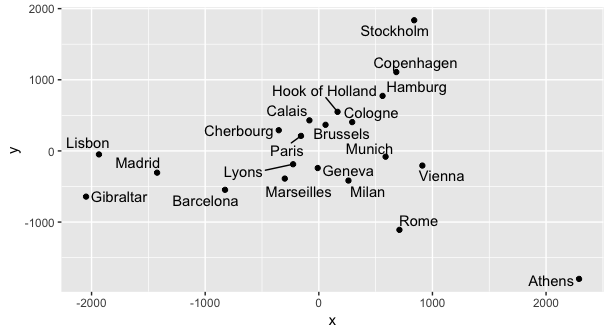
\includegraphics[scale = 0.5]{./images/europ_cities.png}
    \caption{MDS on the Eurepean cities.}
    \label{europ_cities}
\end{figure}

%\indent MDS methods can be divided into two groups: \textit{Metric MDS} and
%\textit{Non-metric MDS}. Metric MDS, also known as \texit{Principal Coordinates Analysis}, 
%uses the differences between similarities. However, Non-metric MDS states that if $a$
%is more similar to $b$ than $c$, then $a$ is closer to $b$ than $c$, but the
%differences between the similarities $ab$ and $ac$ do not have any 
%interpretation. This thesis is focused on the Metric MDS.

\section{Principal coordinates}
Given a matrix \textbf{X} $n \times p$, the matrix of $n$ 
individuals over $p$ variables, it is possible to obtain a new one with 
mean equal to 0 by column from the previous one:

\[
\mathbf{\widetilde{X}} = \Big( \mathbf{I} - \frac{1}{n} \mathbf{1}\mathbf{1'}\Big) \mathbf{X} = \mathbf{P}\mathbf{X},
\]
where 

\[
\mathbf{P} = \Big( \mathbf{I} - \frac{1}{n} \mathbf{1}\mathbf{1'}\Big).
\]

\indent This new matrix, $\mathbf{\widetilde{X}}$, has the same dimensions as 
the orginial one but its columns mean is \textbf{0}. From this matrix, it is 
possible to build two square semi-positive definite matrices: the covariance 
matrix \textbf{S}, defined as $\mathbf{\widetilde{X}'}\mathbf{\widetilde{X}}/n$ 
and the cross-prodructs matrix $Q = \mathbf{\widetilde{X}}\mathbf{\widetilde{X}'}$. 
The last matrix can be interpreted as a similarity matrix between the $n$ elements. 
The term $ij$ is obtained as follows:

\begin{equation} \label{qij}
q_{ij} = \sum_{s=1}^{p} x_{is}x_{js} = \mathbf{x_i'} \mathbf{x_j}
\end{equation}
where $\mathbf{x_i'}$ is the i-th row from $\mathbf{\widetilde{X}}$. 
Given the scalar product formula, ${\mathbf{x_i'}\mathbf{x_j} =  \mid \mathbf{x_i} \mid \mid \mathbf{x_i} \mid \cos\theta_{ij}}$,
if the elements $i$ and $j$ have similar coordinates, then $\cos\theta_{ij} \simeq 1$
and $q_{ij}$ will be large. On the contrary, if the elements are very different,
then $\cos \theta_{ij} \simeq 0$ and $q_{ij}$ will be small. So, 
$\mathbf{\widetilde{X}}\mathbf{\widetilde{X}'}$ can be interpreted as the similarity
matrix between the elements.

\indent The distances between elements can be deduced from the similarity 
matrix. The Eucliden distance between two elements is calculated in the 
following way:

\begin{equation} \label{dij}
d^2_{ij} =  \sum_{s=1}^{p} (x_{is}- x_{js} )^2  = \sum_{s=1}^{p}x_{is}^2 + \sum_{s=1}^p x_{js}^2 - 2\sum_{s=1}^{p} x_{is}x_{js}.
\end{equation}

\indent This expression can be obtained directly from the matrix \textbf{Q}:

\begin{equation} \label{dfromq}
d^2_{ij} = q_{ii} + q_{jj} - 2q_{ij}.
\end{equation}

\indent We have just seen that, given the matrix $\mathbf{\widetilde{X}}$, 
it is possible to get the similarity matrix 
$\mathbf{Q} = \mathbf{\widetilde{X}}\mathbf{\widetilde{X}'}$ and from it, 
to get the distance matrix \textbf{D}. Let $\diag(\mathbf{Q})$ be the
vector that contains the diagonal terms of \textbf{Q} and \textbf{1} be the vector
of ones, the matrix \textbf{D} is given by

\[
\mathbf{D} = \diag(\mathbf{Q}) \mathbf{1}' + \mathbf{1}\diag(\mathbf{Q})' - 2\mathbf{Q}.
\]

\indent The problem we are dealing with goes in the opposite direction. We want 
to rebuild $\mathbf{\widetilde{X}}$ from a square distance matrix \textbf{D}, 
with elements $d_{ij}^2$. The first step is to obtain \textbf{Q} and afterwards, 
to get $\mathbf{\widetilde{X}}$. The theory needed to get the solution can be 
found in \cite{pena_libro}. Here, we summarise it.

\indent The first step is to find out a way to obtain the matrix \textbf{Q} 
given \textbf{D}. We can assume without loss of generality that the mean of 
the variables is equal to 0. This is a consequence of the fact that the distance 
between two points remains the same if the variables are expressed in terms 
of the mean:


\begin{equation} \label{dtraslated}
d_{ij}^2 = \sum_{s = 1}^p (x_{is} - x_{js})^2 = \sum_{s=1} ^p [(x_{is} - \overline{x_s})- (x_{js} - \overline{x_s})]^2.
\end{equation}

\indent The previous condition means that we are lookig for a matrix  
$\mathbf{\widetilde{X}}$ such that $\mathbf{\widetilde{X}'}\mathbf{1} = 0$. 
It also means that $\mathbf{Q}\mathbf{1} = 0$, i.e, the sum of all the elements 
of a column of \textbf{Q} is 0. Since the matrix is symmetric, the previous 
condition should state for the rows as well. 

\indent To establish these constrains, we sum up (\ref{dfromq}) at row level:

\begin{equation} \label{sumrows}
\sum_{i = 1}^n d_{ij}^2 = \sum_{i = 1}^n q_{ii} + nq_{jj} = t + nq_{jj}
\end{equation}
where $t = \sum_{i = 1}^n q_{ii} = \Tr(\mathbf{Q})$, and we have used that the
condition \textbf{Q}\textbf{1} = 0 implies $\sum_{i = 1}^n q_{ij} = 0$. Summing 
up (\ref{dfromq}) at column level:

\begin{equation} \label{sumcols}
\sum_{j = 1}^n d_{ij}^2 = t + nq_{ii}.
\end{equation}

\indent Summing up (\ref{sumrows}) we obtain:

\begin{equation} \label{doublesum}
\sum_{i = 1}^n\sum_{j = 1}^n d_{ij}^2 = 2nt
\end{equation}

\indent Replacing in (\ref{dfromq}) $q_{jj}$ obtained in (\ref{sumrows}) and $q_{ii}$
obtained in (\ref{sumcols}), we have the following expression:

\begin{equation} \label{generaldij}
d_{ij}^2 = \frac{1}{n}\sum_{i = 1}^n d_{ij}^2 - \frac{t}{n} + \frac{1}{n} \sum_{j = 1}^n d_{ij}^2 -\frac{t}{n} -2q_{ij}
\end{equation}

\indent Let $d_{i.}^2 = \frac{1}{n}\sum_{j = 1}^n d_{ij}^2$ and $d_{.j}^2 = \frac{1}{n}\sum_{i=1}^n d_{ij}^2$ 
be the row-mean and column-mean of the elements of \textbf{D}. Using 
(\ref{doublesum}), we have that

\begin{equation} \label{dmeans}
d_{ij}^2 = d_{i.}^2 + d_{.j}^2 - d_{..}^2-2q_{ij}
\end{equation}
where $d_{..}$ is the mean of all the elements of \textbf{D}, given by

\[
d_{..}^2 = \frac{1}{n^2}\sum \sum d_{ij}^2.
\]

\indent Finally, from (\ref{dmeans}) we get the expression:

\begin{equation} \label{qij2}
q_{ij} = -\frac{1}{2}(d_{ij}^2 - d_{i.}^2 - d_{.j}^2 + d_{..}^2).
\end{equation}

\indent The previous expression shows how to build the matrix of similarities 
\textbf{Q} from the distance matrix \textbf{D}.

\indent The next step is to obtain the matrix \textbf{X} given the matrix 
\textbf{Q}. Let's assume that the similarity matrix is positive definite of 
range $p$. Therefore, it can be represented as

\[
\mathbf{Q} = \mathbf{V}\mathbf{\Lambda}\mathbf{V'}
\]
where $\mathbf{V}$ is a $n \times p$ matrix that contains the eigenvectors with
not nulls eigenvalues of \textbf{Q}. $\mathbf{\Lambda}$ is a diagonal matrix 
$p \times p$ that contains the eigenvalues.

\indent Re-writing the previous expression, we obtain

\begin{equation} \label{generalQ}
\mathbf{Q} = (\mathbf{V}\mathbf{\Lambda}^{1/2})(\mathbf{\Lambda}^{1/2}\mathbf{V'}).
\end{equation}

Getting

\[
\mathbf{Y} = \mathbf{V}\mathbf{\Lambda}^{1/2}.
\]

We have obtained a matrix with dimensions $n \times p$ with $p$ uncorrelated
variables that reproduce the initial metric. It is important to notice that if 
one starts from \textbf{X} (i.e \textbf{X} is known) and calculates from these
variables the distance matrix in (\ref{dij}) and after that it is applied
the method explained, the matrix obtained is not the same as \textbf{X}, but
its principal components. This happens since the distance between the rows in
a matrix does not change if:

\begin{itemize}
\item The row-mean values are modified by adding the same row vector to all
the rows in \textbf{X}.
\item Rows are rotated, i.e, \textbf{X} is postmultiplied by an orthogonal 
matrix.
\end{itemize}

\indent By (\ref{dfromq}), the distance is a function of the terms of the 
similarity matrix \textbf{Q} and this matrix is invariant given any rotation,
reflexion or translation of the variables

\[
\mathbf{Q} = \mathbf{\widetilde{X}} \mathbf{\widetilde{X'}} = \mathbf{\widetilde{X}} \mathbf{A} \mathbf{A'}\mathbf{\widetilde{X'}}
\]
for any orthogonal \textbf{A} matrix. The matrix \textbf{Q} only contains 
information about the space generated by the variables \textbf{X}. Any rotation,
reflexion or translation keeps the distance unchaged. Therefore, the solution
is not unique.


\section{Building principal coordinates}
%In general, the distance matrix is not compatible with an Eucliden metric but
%usually the similarity matrix obtained from it has $p$ positive eigenvalues  
%which are greater than the other ones. If the rest $n-p$ of not null eigenvalues 
%are much less than the other ones, it is possible to obtain an (approximated)
%representation using the $p$ eigenvectors associated with the first $p$
%eigenvalues of the similarity matrix. 

\indent Let \textbf{D} be a square distance matrix. The process to obtain 
the \textit{principal coordinates} is:

\begin{enumerate}
\item Build the matrix $\mathbf{Q = - \frac{1}{2} PDP}$ of cross-products.
\item Obtain the eigenvalues of \textbf{Q}. Take the $r$ greatest eigenvalues. 
Since $\mathbf{P1}=0$, where \textbf{1} is a vector of ones, 
$\range(\mathbf{Q})=n-1$, being the vector \textbf{1} an eigenvector with 
eigenvalue 0. 
\item Obtain the coordinates of the rows in the variables 
$\mathbf{v_i}\sqrt{\lambda_i}$,
where $\lambda_i$ is an eigenvalue of \textbf{Q} and $\mathbf{v_i}$ is the
associated unitary eigenvector. This implies that \textbf{Q} is apporximated by:

\[
\mathbf{Q} \approx (\mathbf{V_r \Lambda}^{1/2})(\mathbf{\Lambda_r}^{1/2} \mathbf{V_r'}).
\]

\item Take as coordinates of the points the following variables:
\[
\mathbf{Y_r} = \mathbf{V_r}\mathbf{\Lambda_r}^{1/2}.
\]
\end{enumerate}

\indent The method can also be applied if the initial information is not a 
distance matrix but a similarity matrix. A \textit{similarity function}, 
$s_{ij}$, between two element $i$ and $j$  is defined as:

\begin{itemize}
\item $s_{ii} = 1$.
\item $0 \leq s_{ij} \leq 1$.
\item $s_{ij} = s_{ji}$.
\end{itemize}

If the initial information is \textbf{Q}, a similariy matrix, then $q_{ii} = 1$,
$q_{ij} = q_{ji}$ and $0 \leq q_{ij} \leq 1$. The associated distance matrix 
is

\[
d_{ij}^2 = q_{ii} + q_{jj} - 2q_{qij} = 2(1-q_{ij}),
\]
and it is easy to see that $\sqrt{2(1-q_{ij})}$ is a distance and it verifies
the triangle inequality.


\section{Procrustes transformation}
As we have mentioned before, the MDS solution is not unique. One example of it 
is shown in Figure (\ref{twosol}).

\begin{figure}[ht]
    \centering
    \subfloat[]{{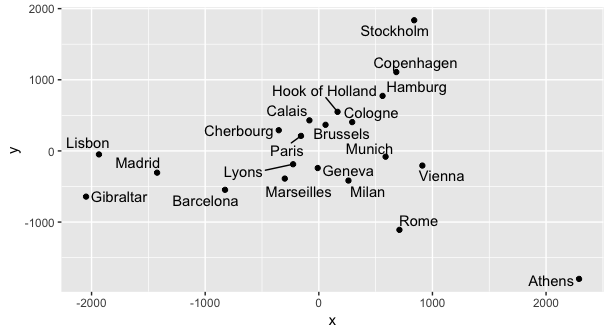
\includegraphics[width=8cm]{./images/europ_cities.png} }}%
    \qquad
    \subfloat[]{{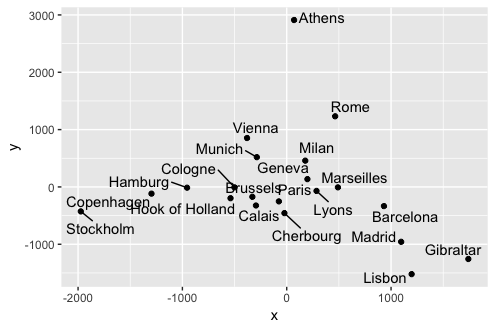
\includegraphics[width=8cm]{./images/europ_cities_rot.png} }}%
    \caption{Two different solutions of MDS.}%
    \label{twosol}%
\end{figure}


\indent Since rotations, translations and reflections are distance-preserving 
functions, one can find two different MDS configurations 
for the same set of data. How is it possible to align both solutions? This 
problem is solved by means of \textit{Procrustes transformations}.  


\indent The Procrustes problem is concern with fitting a configuration (testee)
to another (target) as closely as possible. In the simple case, both 
configurations have the same dimensionality and the same number of points, which
can be brought into 1-1 correspondence by substantive considerations. Under
orthogonal transformations, the testee can be fitted it to the target. In 
addition to such rigid motions, one may also allow for dilations and for shifts.

\indent All the details are developed in  \cite{BorgGroenen2005}. This is out 
of the scope of this thesis. However, since it has been a repeatdly used tool, 
we briefly summarise it. 

\indent Let \textbf{A} and \textbf{B} be two different MDS configurations for
the same set of data. Without loss of generality, let's assume that the target 
is \textbf{A} and the testee is \textbf{B}. One wants to obtain $s$, \textbf{T}
and \textit{t} such that

\[
\mathbf{A} = s \mathbf{B} \mathbf{T} + \mathbf{1t}'
\]
where \textbf{T} is an orthogonal matrix. As mentioned before, 
in \cite{BorgGroenen2005} are all the details needed to estimate 
these parameters.

\section{Multidimensional Scaling with \textsf{R}}

All the algorithms have been coded in \textsf{R}, since it has a widely 
statistics packages already implemented. We have used two packages for 
developing our MDS approaches:

\begin{itemize}
\item Package: \textsf{stats}. From this one we have used the function 
\textsf{cmdscale} to do the MDS. The output of this function is:
\begin{itemize}
\item The new coordinates for the individuals.
\item All the eigenvalues found.
\end{itemize}
\item Package: \textsf{MCMCpack}. From this one we have used the function 
\textsf{procrustes} to do the Procrustes transformation. The output of 
this function is:
\begin{itemize}
\item The dilation coeficient $s$.
\item The orthogonal matrix \textbf{T}.
\item The translation vector \textbf{t}.
\end{itemize}
\end{itemize}

\chapter{Algorithms for Multidimensional Scaling with Big Data}

\section{Why is it needed?}
In this chapter we present the algorithms developed so that MDS can be applied
when we are dealing with large datasets. The natural question here is why we need 
them if there are already some implementations. To answer this question, let's 
take a look at the Figures (\ref{elapsed_time_mds}) and (\ref{memory_distance}).

 
\begin{figure}[ht]
\centering
    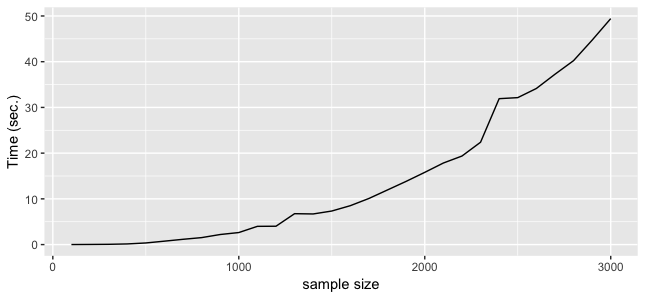
\includegraphics[scale = 0.5]{./images/elapsed_time_mds.png}
    \caption{Elapsed time to compute MDS.}
    \label{elapsed_time_mds}
\end{figure}



\begin{figure}[ht]
\centering
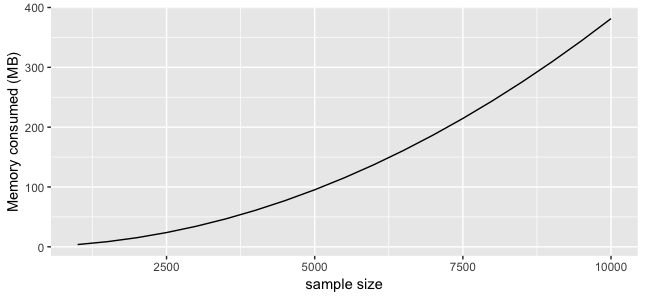
\includegraphics[scale = 0.5]{./images/memory_distance.png}
\caption{Memory consumed to compute distance.}
\label{memory_distance}
\end{figure}


\indent Figure (\ref{elapsed_time_mds}) shows the time needed to compute MDS
as a function of the sample size. As we can see, the time grows 
exponentially. Apart of the time issue, there is another one related to the
memory needed to compute the distance matrix. Figure (\ref{memory_distance}) 
points out that it is required at least 400MB to store the distance 
matrix when the dataset is close to 10.000 observations.

\indent In order to solve these problems, we have developed three algorithms:


\begin{itemize}
\item \textit{Divide and Conquer MDS:} Before this thesis, 
\textit{Pedro Delicado} had done some work about  MDS with big
datasets and he had already created a first approach, which is this one. The 
algorithm is based on the idea of dividng and conquering. Given a big data set, 
it is divided into $p$ small ones, then MDS is perform over all the partitions
and finally the $p$ solutions are stitched so that all the points lie on the 
same system of coordinates.

\item \textit{Fast MDS:} during the phase of gathering information, we found an 
article that solved the problem of scalability \cite{Yang06afast}. The 
authors  use a divide and conquer idea together with recursive programming. 

\item \textit{MDS based on Gower interpolation formula:} this algorithm uses
Gower interpolation formula which allows to add a new set of points
to an existing MDS configuration \cite{gowerformula}. 

\end{itemize}

In the next sections we are going to provide a description of the algorithms. 
If further details about the implementation are needed, the code is provided in 
\autoref{chap:code}.

\section{Divde and Conquer Multidimensional Scaling}

\begin{itemize}

\item The first step is to divide the original dataset into $p$ partitions: 
$\mathbf{X_1},\dots, \mathbf{X_p}$. The number of partitions, $p$, is also
the number of steps needed to compute the algorithm.

\item Calculate the MDS for the first partition: \textbf{MDS(1)}. This solution
will be used as a guide to align the MDS for the remaining partitions. We will 
use a new variable, \textbf{cum-mds}, that will be growing as long as new 
partitions are used. Before adding a new MDS, it will be aligned and, after 
that, added. 

\item Define \textbf{cum-mds} equal to \textbf{MDS(1)} and start iterating 
until the last partition is reached.

\item Given a step $k$, $1 < k \leq p$, partitions $k$ and \textit{k-1} are 
joint, i.e, $\mathbf{X_k} \cup \mathbf{X_{k_1}}$. MDS is calculated on 
this union, obtaining $\mathbf{MDS_{k, k-1}}$. In order to append the
rows of the \textit{k-th} partition to \textbf{cum-mds}, the following steps 
are performed:

\begin{itemize}
\item Take the rows of the partition \textit{k-1} from $\mathbf{MDS_{k, k-1}}$: 
$\mathbf{MDS_{k, k-1}} \Bigr|_{k-1}$.
\item Take the rows of the partition \textit{k-1} from \textbf{cum-mds}: 
\textbf{cum-mds} $\Bigr|_{k-1}$.
\item Apply Procrustes to align both solutions. It means that a scalar number
\textit{s}, a vector \textbf{t} and an orthogonal matrix \textbf{T} are obtained
so that
\[
\boldsymbol{\cummds} \Bigr|_{k-1} = s \mathbf{MDS_{k, k-1}} \Bigr|_{k-1} \mathbf{T} + \mathbf{1t}'.
\]
\item Take the rows of the partition $k$ from $\mathbf{MDS_{k, k-1}}: \mathbf{MDS_{k, k-1}} \Bigr|_{k}$.
\item Use the previous Procrustes parameters to append the rows of 
$\mathbf{MDS_{k, k-1}} \Bigr|_{k}$ with \textbf{cum-mds}:
\[
\boldsymbol{\cummds} \Bigr|_{k} := s \mathbf{\mathbf{MDS_{k, k-1}}} \Bigr|_{k} \mathbf{T} + \mathbf{1t}'.
\]
\item Add the previous dataset to \textbf{cum-mds}, i.e:
\[
\boldsymbol{\cummds} = \boldsymbol{\cummds} \bigcup \boldsymbol{{\cummds}} \Bigr|_{k}
\]

\end{itemize}
\end{itemize}

As we have seen, the algorithm depends on $p$, the number of partitions. How 
many of them are needed? To answer this question, Let $l \times l$ be the largest 
matrix that allows to run MDS eficiently. If $n$ is the number of rows 
of \textbf{X}, then $p$ is $\frac{2n}{l}$. 

\section{Fast Multidimensional Scaling}




\section{Multidimensional Scaling based on Gower interpolation}



\chapter{Simulation study}
%Decir que siempre he usado la misma maquina

\chapter{Conclusions}

%\bibliographystyle{unsrt}
\bibliographystyle{chicago}
\bibliography{bibliography.bib}


\appendix 

\chapter{Code}
\label{chap:code}

\chapter{Problems encountered during the development}
% Los paquetes de R que existen y sus limitaciones
% Para alinear las soluciones --> procrustes
% Lo complicado que me resulto implementar el fast

\end{document}


% Notacion:
%%% Matrices: mayusculas y negritas
%%% Vectores: minusculas y negritas
%%% constantes: minusculas y normal

% To do:
%%% Mencionar a Roger




%\subsection{Algorithm}
%\begin{algorithm}[H]
%  \SetAlgoLined
%  \SetKwInOut{Input}{input}
%  \SetKwInOut{Output}{output}
%   \Input{x: (matrix) a dataset. \newline 
%   l: (integer) the largest matrix dimension that allows MDS to be executed eficiently. \newline
%   s: (integer) the estimated dimensionality of the matrx.
%  }
%  \Output{
%    The output is a list of two elements: \newline
%    points: (matrix) MDS configuration. \newline
%    eigen: (vector) The eigenvalues. \newline
%  }
%  {$ls_positions = list()$} \Comment*[r]{This list will contain the positions of the rows per each partition}
%  {$list_eigenvalues = list()$} \Comment*[r]{This list will contain the eigenvalues}
%  {$i_eigen = 1$};
%  {$p = ceiling(2*nrow(x)/l)$} \Comment*[r]{Total partitions}
%  {$groups = sample(x = p, size = nrow(x), replace = TRUE)$}
%  groups = sort(groups)
%  \While{not at end of this document}{
%    read current\;
%    \eIf{understand}{
%      go to next section \Comment*[r]{Some comment}
%      current section becomes this one\;
%    }{
%      go back to the beginning of current section\;
%    }
%  }
%  \caption{How to write algorithms}
%\end{algorithm}
